\documentclass[12pt]{report}
\usepackage[utf8]{inputenc}
\usepackage[russian]{babel}
%\usepackage[14pt]{extsizes}
\usepackage{listings}
\usepackage{graphicx}
\usepackage{amsmath,amsfonts,amssymb,amsthm,mathtools} 
\usepackage{pgfplots}
\usepackage{filecontents}
\usepackage{indentfirst}
\usepackage{eucal}
\usepackage{amsmath}
\usepackage{enumitem}
\frenchspacing

\usepackage{indentfirst} % Красная строка


%\usetikzlibrary{datavisualization}
%\usetikzlibrary{datavisualization.formats.functions}

\usepackage{amsmath}


% Для листинга кода:
\lstset{ %
language=caml,                 % выбор языка для подсветки (здесь это С)
basicstyle=\small\sffamily, % размер и начертание шрифта для подсветки кода
numbers=left,               % где поставить нумерацию строк (слева\справа)
numberstyle=\tiny,           % размер шрифта для номеров строк
stepnumber=1,                   % размер шага между двумя номерами строк
numbersep=5pt,                % как далеко отстоят номера строк от подсвечиваемого кода
showspaces=false,            % показывать или нет пробелы специальными отступами
showstringspaces=false,      % показывать или нет пробелы в строках
showtabs=false,             % показывать или нет табуляцию в строках
frame=single,              % рисовать рамку вокруг кода
tabsize=2,                 % размер табуляции по умолчанию равен 2 пробелам
captionpos=t,              % позиция заголовка вверху [t] или внизу [b] 
breaklines=true,           % автоматически переносить строки (да\нет)
breakatwhitespace=false, % переносить строки только если есть пробел
escapeinside={\#*}{*)}   % если нужно добавить комментарии в коде
}

\usepackage[left=2cm,right=2cm, top=2cm,bottom=2cm,bindingoffset=0cm]{geometry}


% plot
\usepackage{pgfplots}
\usepackage{filecontents}
\usetikzlibrary{datavisualization}
\usetikzlibrary{datavisualization.formats.functions}

\graphicspath{ {img/} }




\begin{document}
	\begin{titlepage}
		\thispagestyle{empty}
		
		\noindent
		\begin{minipage}{0.15\textwidth}
			
\includegraphics[width=\linewidth]{main_logo}
		\end{minipage}
		\noindent
		\begin{minipage}{0.9\textwidth}
			\centering
			\textbf{Министерство науки и высшего образования Российской Федерации}\\
			\textbf{Федеральное государственное бюджетное образовательное учреждение высшего образования}\\
			\textbf{«Московский государственный технический университет имени Н.Э.~Баумана}\\
			\textbf{(национальный исследовательский университет)»}\\
			\textbf{(МГТУ им. Н.Э.~Баумана)}
		\end{minipage}
		
		\noindent
		\rule{18cm}{3pt} %пустая строка
		\newline\newline %пустая строка
		\noindent ФАКУЛЬТЕТ $\underline{\text{«Информатика и системы управления»}}$ \newline\newline
		\noindent КАФЕДРА $\underline{\text{«Программное обеспечение ЭВМ и информационные технологии»}}$\newline\newline\newline\newline\newline
		
		
		\begin{center}
			\noindent\begin{minipage}{1.3\textwidth}\centering
				\Large\textbf{  Отчёт о лабораторной работе №3}\newline
				\textbf{по дисциплине "Анализ алгоритмов"}\newline
				\textbf{на тему "Алгоритмы сортировки"}\newline\newline
			\end{minipage}
		\end{center}
		
		\noindent\textbf{Студент} $\underline{\text{Коняев Е.А}}$\newline\newline
		\noindent\textbf{Группа} $\underline{\text{ИУ7-53Б}}$\newline\newline
		\noindent\textbf{Преподаватели} $\underline{\text{Волкова Л.Л., Строганов Ю.В.}}$\newline\newline
		\noindent\textbf{Дата сдачи отчета}$\underline{\text{~~~~~~~~~~~~~~~~~~~~~~~~~~~}}$\newline\newline
		\noindent\textbf{Оценка (баллы)} $\underline{\text{~~~~~~~~~~~~~~~~~~~~~~~~~~~}}$\newline\newline\newline
		
		\begin{center}
			\vfill
			Москва~---~\the\year~г.
		\end{center}
	\end{titlepage}
	
	\setcounter{page}{2}
	\tableofcontents
	
	\newpage
	\chapter*{Введение}
	
	\addcontentsline{toc}{chapter}{Введение}
	
	
Алгоритмы сортировки — это набор инструкций, которые принимают массив или список в качестве входных данных и упорядочивают элементы в определенном порядке. Сортировка чаще всего осуществляется в числовом или алфавитном (или лексикографическом) порядке и может быть в порядке возрастания (A-Z, 0-9) или убывания (Z-A, 9-0).

Сортировки важны потому что они часто могут уменьшить сложность решаемой задачи, а потому алгоритмы сортировки очень важны в компьютерных науках. Эти алгоритмы имеют прямое применение в алгоритмах поиска, алгоритмах баз данных, методах разделяй и властвуй, алгоритмах структуры данных и многом другом.\newline\newline
При выборе алгоритма сортировки необходимо учитывать: 
\begin{enumerate}
	\item количиество сортируемых элементов;
	\item количество доступной памяти;
	\item возможность увеличения коллекции с сортируемыми элементами.
\end{enumerate}
  

Эти факторы могут определить, какой алгоритм будет работать лучше всего в каждой ситуации. Некоторым алгоритмам может потребоваться много места или памяти для запуска, в то время как другим, при том, что они не являются самыми быстрыми, не требуется много ресурсов для запуска.

Именно из-за разнообразия алгоритмов сортровок, их особенностей и областей применения, данная работа была посвещена анализу некоторых из этих алгоритмов.
	
	
	

	
	\chapter{Аналитическая часть}
	
	\section{Цели и задачи}
	
	Целью данной работой является исследования алгоритмов сортировок пузырьком, вставками и выбором. Для этого в ходе исследования алгоритмов требуется решить следующие задачи:
	\begin{enumerate}
		\item изучить и рассмотреть выбранный алгоритмы сортировок;
		\item построить блок-схемы выбранных алгоритмов;
		\item реализовать каждый из алгоритмов;
		\item рассчитать их трудоемкость;
		\item эксперитментально оценить временные характеристики алгоритмов;
		\item сделать вывод на основании проделанной работы.
	\end{enumerate}
	
	
	\section{Сортировка пузырьком}
	
	 Сортировка пузырьком — это базовый алгоритм для упорядочивания массива чисел или других элементов в правильном порядке. Метод работает, проверяя каждый набор соседних элементов в строке слева направо, меняя их позиции, если они не в порядке (не в порядке возрастания/убывания). 
	 
	 Алгоритм будет просматривать два элемента за раз, переставлять те, которые еще не в порядке возрастания/убывания, слева направо, а затем продолжать циклически проходить всю последовательность N - 1 раз, где N - кол-во элементов массива. 
	 
	 Существует так же модифицированная версия данного алгоритма, где процесс прохода по всем элементам массива продолжается до тех пор, пока алгоритм не посмотрит весь набор чисел и не найдет двух элементов, которые нужно поменять местами.
	
	\section{Сортировка вставками}
	
	В ходе данного алгоритма происходит прохождение по сортируемому массиву слева направо и обрабатывае по очереди каждого элемента. Слева от очередного элемента увеличивается отсортированная часть массива, справа по мере процесса сортировки постепенно уменьшается неотсортированная часть. В отсортированной части массива ищется точка вставки для очередного элемента. Сам элемент отправляется в буфер, в результате чего в массиве появляется свободная ячейка — это позволяет сдвинуть элементы и освободить точку вставки.
	
	\section{Сортировка выбором}
	
	Идея данного метода сортировки состоит в том, чтобы создавать отсортированную последовательность путем присоединения к ней одного элемента за другим в правильном порядке. Можно строить готовую последовательность, начиная с левого конца массива. Алгоритм состоит из n последовательных шагов. На очередном шаге выбираем наименьший из элементов, начинаю текущим и заканчивая последним, и меняем его местами с очередным элементом.
	
	Таким образом, на последнем шаге вся последовательность, кроме последнего элемента оказывается отсортированной, а последний элемент в свою очередь стоит на последнем месте корректно потому, что все меньшие элементы уже ушли влево.
	
	\section{Вывод}
	
	В данном разделе были рассмотрены 3 алгоритма сортировки: пузырьком, вставками и выбором.
	
	\clearpage
	
	\chapter{Конструкторская часть}
	
	\section{Схемы алгоритмов}
	
	На рисунках \ref{fig:schema_bubble}, \ref{fig:schema_selection} и \ref{fig:schema_insertion} показаны схемы алгоритмов сортировки пузырьком, выбором и вставками соответственно.
	
	\begin{figure}[h]
		\centering
		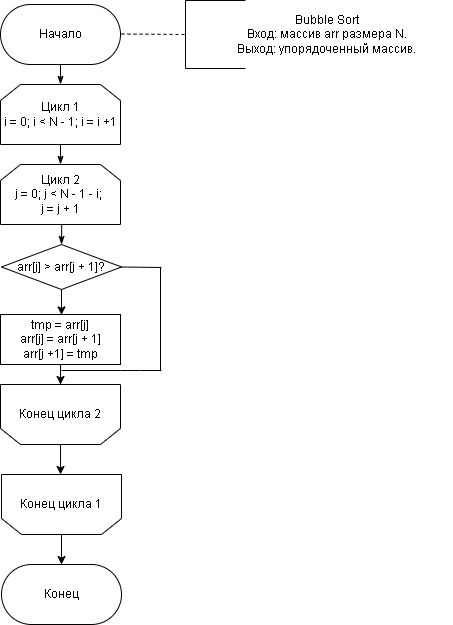
\includegraphics[width=0.9\linewidth]{bubble}
		\caption{Схема сортировки пузырьком}
		\label{fig:schema_bubble}
	\end{figure}
	
	\begin{figure}[h]
		\centering
		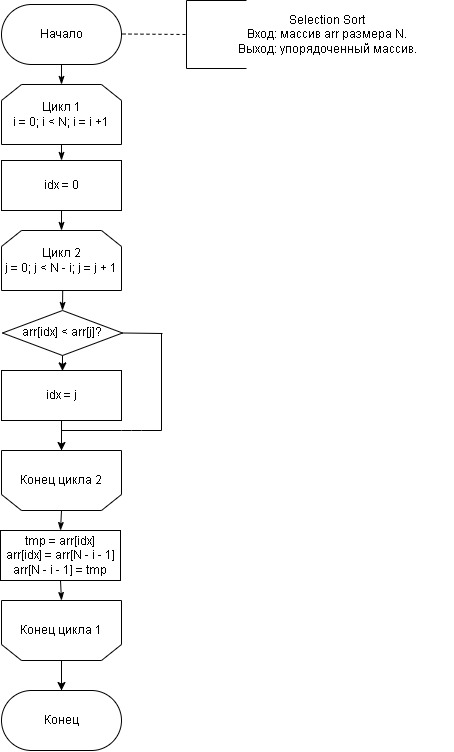
\includegraphics[width=0.9\linewidth]{selection}
		\caption{Схема сортировки выбором}
		\label{fig:schema_selection}
	\end{figure}
	
	\begin{figure}[h]
		\centering
		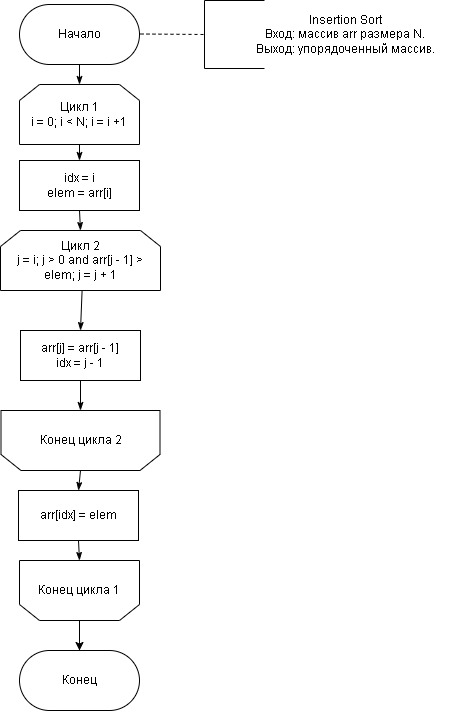
\includegraphics[width=0.9\linewidth]{insertion}
		\caption{Схема сортировки вставками}
		\label{fig:schema_insertion}
	\end{figure}
	
	\section{Вывод}
	
	В данном разделе на основе теоретических данных, полученных в аналитическом разделе были разработаны схемы алгоримов трех рассматриваемых алгоритмов сортировок.
	
	\chapter{Технологическая часть}
	
	В данном разделе преведены требования к ПО, обоснования выбора языка программирования, среды разработки, приведен способ замера времени выполнения, а так же приведены листинги кода.
	
	\section{Требования к ПО}
	
	В программе должна присутсвовать возможность :
	
	\begin{enumerate}
		\item указания размера входного массива, а так же его элементов;
		\item сортировки входного массива одним из трех рассматриваемых способов сортировок;
		\item проверки временных характеристик на разных типах входных массивов (упорядочен по возрастанию/убыванию, заполнен случайными числами), для рассматриваемых способов сортировок.
	\end{enumerate}
	
	\section{Выбор языка программирования и среды разработки}
	
	Для реализации трех алгоритмов сортировок был выбор язык С, так как я уже знаком с данным языком и поставленная задача будет решена максимально быстро.

	Средой разработки был выбран СLion. Данный выбор обусловлен тем, что данная среда на сегодняшний момент является по-моему мнению самой удобной IDE для разработки под C/C++, в силу того, что предоставляет мощные инструменты для отладки кода и его быстрого написания. 
	
	\section{Выбор библиотеки и способа для замера времени}
		Для замера времени выполнения сортировок использовалась стандартная функция библиотеки <time.h> языка С~---~clock(), которая замеряет процессорное время. Если измерить время перед началом выполнения алгоритма, и после его окончания, то можно получить время выполнения функции. Реализация данной функции привидена в списке литературы[1].
		
		Посколько все процессорное время не отдается какоЙ-либо одной задаче (явление вытеснения процессов из ядра, квантование процессорного времени), то усреднить результаты вычислений: замерить совокупное время выполнения реализации алгоритма N раз и вычислить среднее время выполнения.
		
	\section{Листинги кода}
	
	В листингах \ref{bubble-code},\ref{selection-code},\ref{insertion-code} приведены листинги алгоритмов сортировок пузырьком, выбором и вставками соответсвенно.
	
	\begin{lstlisting}[label=bubble-code,caption=Функция сортировки массива пузырьком,language=C]
		void bubbleSort(int *arr, size_t n)
		{
			for (int i = 0; i < n - 1; ++i)
			for (int j = 0; j < n - 1 - i; ++j) {
				if (arr[j] > arr[j + 1])
				{
					int tmp = arr[j];
					arr[j] = arr[j + 1];
					arr[j + 1] = tmp;
				}
			}
		}
	\end{lstlisting}

	
	\begin{lstlisting}[label=selection-code,caption=Функция сортировки массива выбором,language=C]
		void selectionSort(int *arr, size_t n)
		{
			for (int i = 0; i < n; ++i) {
				int idxToSwap = 0;
				for (int j = 0; j < n - i; ++j) {
					if (arr[idxToSwap] < arr[j]) {
						idxToSwap = j;
					}
				}
				int tmp = arr[idxToSwap];
				arr[idxToSwap] = arr[n - i - 1];
				arr[n - i - 1] = tmp;
			}
		}
	\end{lstlisting}

	\begin{lstlisting}[label=insertion-code,caption=Функция сортировки массива вставками,language=C]
		int insertionSort(int *arr, size_t n)
		{
			for (int i = 0; i < n; ++i) {
				int idxInsert = i;
				int insertElement = arr[i];
				for (int j = i; j > 0 && arr[j - 1] > insertElement; --j) {
					arr[j] = arr[j - 1];
					idxInsert = j - 1;
				}
				arr[idxInsert] = insertElement;
			}
		}
	\end{lstlisting}

	\section{Тестирование алгоритмов}

	В таблице~\ref{tbl:test} приведены тесты для функций, реализующих алгоритмы сортировки. Все тесты пройдены успешно.
	
	\begin{table}[h!]
		\begin{center}
			\begin{tabular}{|c|c|c|}
				\hline
				Входной массив & Результат & Ожидаемый результат \\ 
				\hline
				$[10, 20, 30, 40, 50]$ & $[10, 20, 30, 40, 50]$  & $[10, 20, 30, 40, 50]$\\\hline
				$[50, 40, 30, 20, 10]$  & $[10, 20, 30, 40, 50]$ & $[10, 20, 30, 40, 50]$\\\hline
				$[-15, -21, -37, -24, -54]$  & $[-54, -37, -24, -21, -15]$  & $[-54, -37, -24, -21, -15]$\\\hline
				$[4]$  & $[4]$  & $[4]$\\\hline
				Пустой массив  & Пустой массив  & Пустой массив\\
				\hline
			\end{tabular}
			\caption{\label{tbl:test}Тестирование функций}
		\end{center}
	\end{table}

	\section{Вывод}
	
	В данном разделе были разработаны исходные коды трёх алгоритмов сортировки: пузырьком, выбором и вставками.
	
	\chapter{Экспериментальная часть}
	
	\section{Технические характеристики}
	
	Ниже приведены технические характеристики устройства, на котором было проведено тестирование ПО:
	
	\begin{enumerate}
		\item Операционная система: Windows-10, 64-bit.
		\item Оперативная память: 16 GB.
		\item Процессор: Intel(R) Core(TM) i7-8565U CPU @ 1.80GHz, 1992 МГц, 4 ядра, 8 логических процессоров
		
		
	\end{enumerate}
	
	\section{Время выполнения алгоритмов}
	
	\begin{table} [h!]
		\caption{Таблица времени выполнения сортировок на данных, отсоритрованных по возрастанию (в мс)}
		\begin{center}
			\begin{tabular}{|c | c | c | c|}
				
				\hline
				
				Размер & bubble & selection & insertion  \\ [0.5ex]
				
				\hline
				
				100 & 0.02 & 0.02 & 0 \\ 
				
				\hline 
				
				1000 & 1.02 & 1.26 & 0 \\ 
				
				\hline 
				
				10000 & 102.5 & 117.5 & 0 \\ 
				
				\hline 
			\end{tabular}
		\end{center}
	\end{table}

	\begin{center}
		\begin{tikzpicture}
				\begin{axis} [
					legend pos = north west,
					grid = major,
					xmin = 0,
					ymin = 0, 
					xmax = 10000,
					ymax = 120,
					xlabel = $\text{кол-во элементов}$,
					ylabel = $\text{время (мс)}$,
					title=$\text{График зависимости времени сортировок от кол-ва элементов на упорядоченном массиве}$
					]
					\legend{ 
						$bubble$, 
						$selection$, 
						$insertion$
					};
					\addplot coordinates {
						(100,0.02) (1000,1.02) (10000,102.5)
					};
					\addplot coordinates {
						(100,0.02) (1000,1.26) (10000,117.5)
					};
					\addplot coordinates {
						(100,0.00) (1000,0) (10000,0)
					};
				\end{axis}
		\end{tikzpicture}
	\end{center}
	
	\begin{table} [h!]
		\caption{Таблица времени выполнения сортировок на данных, отсоритрованных по убыванию (в мс)}
		\begin{center}
			\begin{tabular}{|c | c | c | c|}
				
				\hline
				
				Размер & bubble & selection & insertion  \\ [0.5ex]
				
				\hline
				
				100 & 0.02 & 0.02 & 0.02 \\ 
				
				\hline 
				
				1000 & 1.94 & 1.04 & 1.48 \\ 
				
				\hline 
				
				10000 & 187.8 & 103.3 & 139.9 \\ 
				
				\hline 
				
			\end{tabular}
		\end{center}
	\end{table}

	\begin{center}
		\begin{tikzpicture}
			\begin{axis} [
				legend pos = north west,
				grid = major,
				xmin = 0,
				ymin = 0, 
				xmax = 10000,
				ymax = 120,
				xlabel = $\text{кол-во элементов}$,
				ylabel = $\text{время (мс)}$,
				title=$\text{График зависимости времени сортировок от кол-ва элементов на обратно упорядоченном массиве}$
				]
				\legend{ 
					$bubble$, 
					$selection$, 
					$insertion$
				};
				\addplot coordinates {
					(100,0.02) (1000,1.94) (10000,187.8)
				};
				\addplot coordinates {
					(100,0.02) (1000,1.04) (10000,103.3)
				};
				\addplot coordinates {
					(100,0.02) (1000,1.48) (10000,139.9)
				};
			\end{axis}
		\end{tikzpicture}
	\end{center}
	
	\begin{table} [h!]
		\caption{Таблица времени выполнения сортировок на случайных данных (в мс)}
		\begin{center}
			\begin{tabular}{|c | c | c | c|}
				
				\hline
				
				Размер & bubble & selection & insertion  \\ [0.5ex]
				
				\hline
				
				100 & 0.02 & 0.02 & 0.02 \\ 
				
				\hline 
				
				1000 & 2.02 & 0.96 & 0.72 \\ 
				
				\hline 
				
				10000 & 229.1 & 86.8 & 69.4 \\ 
				
				\hline 
				
			\end{tabular}
		\end{center}
	\end{table}

	\begin{center}
		\begin{tikzpicture}
			\begin{axis} [
				legend pos = north west,
				grid = major,
				xmin = 0,
				ymin = 0, 
				xmax = 10000,
				ymax = 120,
				xlabel = $\text{кол-во элементов}$,
				ylabel = $\text{время (мс)}$,
				title=$\text{График зависимости времени сортировок от кол-ва элементов на массиве случайных чисел}$
				]
				\legend{ 
					$bubble$, 
					$selection$, 
					$insertion$
				};
				\addplot coordinates {
					(100,0.02) (1000,2.02) (10000,229.1)
				};
				\addplot coordinates {
					(100,0.02) (1000,0.96) (10000,86.8)
				};
				\addplot coordinates {
					(100,0.02) (1000,0.72) (10000,69.4)
				};
			\end{axis}
		\end{tikzpicture}
	\end{center}

	\section{Вывод}
	
	Алгоритм сортировки вставками работает лучше сортировок выбором и пуззырьком на случайных и уже отсортированных числах. Сортировка вставками массива из 10000 элементов в 3.3 раза быстрее сортировки пузырььком и в 1.6 раз ьыстрее сортировки выбором. Следовательно, алгоритм сортировки вставками работает быстрее, чем алгоритм сортировки пузырьком и выбором на больших массивах данных.
	
	\chapter*{Заключение}
	
	В рамках данной лабораторной работы:
	
	\begin{enumerate}
		\item были изучены и рассмотрены алгоритмы сортировок пузырьком, вставками и выбором;
		\item были построены блок-схемы выбранных алгоритмов;
		\item был реализован каждый из алгоритмов;
		\item была рассчитана их трудоемкость;
		\item были эксперитментально оценены временные характеристики алгоритмов;
		\item были сделаны выводы на основании проделанной работы
	\end{enumerate}
	
	На основании анализа трудоемкости алгоритмов в выбранной модели вычислений, было показано, что алгоритм сортировки вставками имеет наименьшую сложность в уже отсортированном массиве, а так же эффективнее работает на массиве размером 10000, обгоняя по скорости алгоритмы пузырьком и выбором.
	
%	\addcontentsline{toc}{chapter}{Литература}
	
%	\bibliographystyle{utf8gost705u}  % стилевой файл для оформления по ГОСТу
	
%	\bibliography{51-biblio}
	
\end{document}
